\section{Geometric Transformation}
\begin{frame}[c]{Geometric Transformations}
    \large
    \begin{columns}
        \column{0.45\textwidth}
        In particular, point cloud classification should be invariant to:
        \begin{itemize}
            \item Translation
            \item Rotation
            \item Scaling (Dilation)
        \end{itemize}
        \column{0.5\textwidth}
        \centering
        \begin{figure}
            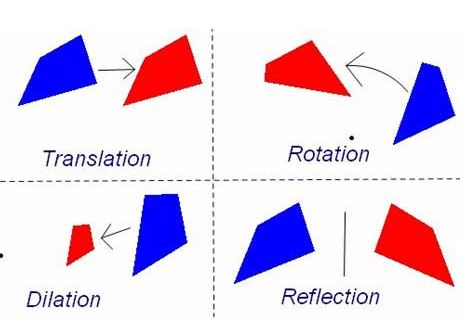
\includegraphics[width=0.8\textwidth]{geometric_transformations}
            \caption{Figure from \cite{BibEntry2019Oct}.}
        \end{figure}
    \end{columns}
    \pnote{
        Relevant: Andere Herausforderung
        \par
        Klassifikation soll unverändert sein über: \\
        - Translation / Bewegung im Raum \\
        - Rotation \\
        - Skalierung \\
        Reflektion sollte bereits über Datensatz enthalten sein
    }
\end{frame}


\begin{frame}[c]{Input Alignment by Transformer Network}
    \begin{columns}
        \column{0.3\textwidth}
        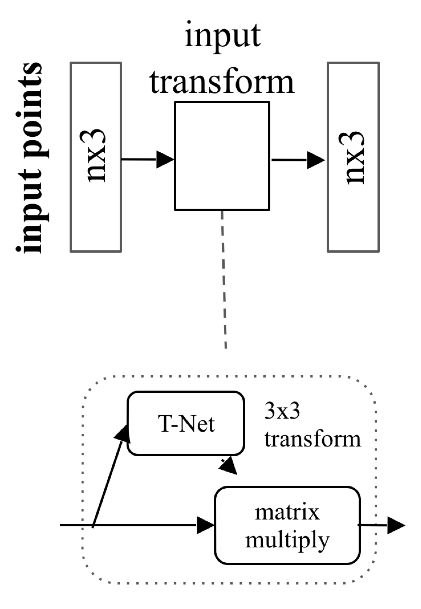
\includegraphics[height=0.7\textheight]{p37_34}
        \column{0.6\textwidth}
        \large
        \pause
        \begin{greenblock}{Solution}
            Have a transformer network (T-Net) figure out data-dependent
            transformations. \\
            \vspace{1em}
            A T-Net is a PointNet (vanilla) with a matrix as output.
        \end{greenblock}
        \vspace{1em}

        \pause
        Additionally, regularize matrix close to orthogonal: $$ L_{reg} = || I - AA^T||_F^2 $$

    \end{columns}
    \blfootnote{Figure from CVPR presentation to \cite{qi2017pointnet}.}
    \pnote{
        Grundidee: Eingabe Normalisieren \\
        Für Point Cloud, Transformation nur Matrixmult
        \par
        PointNet: symmetrisch allgemeiner Funktionsapproximator
        \par
        Verwendung, um datenabhängige Transformationsmatrix \\
        (Normalisierung auf Kanonischen 1-Cube) zu generieren.
    }
\end{frame}


\begin{frame}[c]{Effects of T-Net and Regularization}
    \begin{columns}
        \column{0.6\textwidth}
        \begin{figure}
            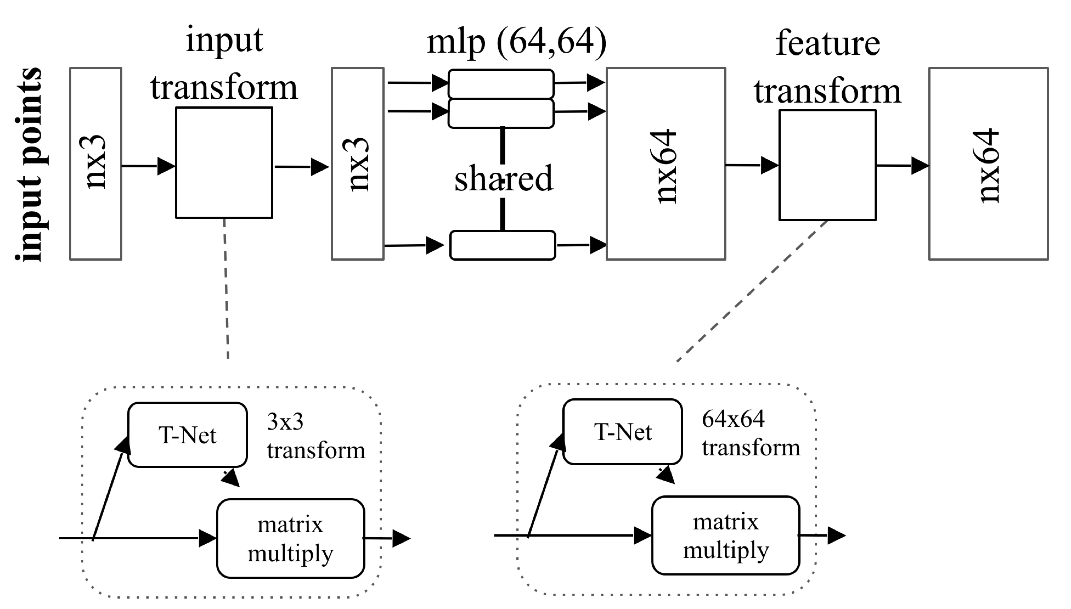
\includegraphics[width=\textwidth,trim=0 10 0 20,clip]{p43_51}
            \caption{Figure from CVPR presentation to \cite{qi2017pointnet}.}
        \end{figure}
        \Large
        \column{0.4\textwidth}
        \pause
        \begin{table}[!ht]
    \centering
    % \resizebox{0.3\textwidth}{!}{%
    \begin{tabular}{l|c}
        Transform & accuracy \\ \hline \hline
        none & 87.1 \\ \hline

        input (3x3) & 87.9 \\
        feature (64x64) & 86.9 \\
        feature (64x64) + reg. & 87.4 \\ \hline

        both & \textbf{89.2}
    \end{tabular}% }
    \caption{
        \textbf{Effects of input feature transforms.} Based on overall classification accuracy on the ModelNet40 \cite{wu20153d} test set.
        Table from \cite{qi2017pointnet}.
    } \label{table:transforms}
\end{table}

    \end{columns}
    \pnote{
        Wir wollen auch mehr als nur die Eingabe Normalisieren \\
        Konkret: Lokaler Feature Vektor  größe 64
    }
\end{frame}

